	\chapter{Conclusiones finales}
\cursi{Nos hemos propuesto resolver un problema que se encuentra en todos los sistemas de procesamiento de señales y los microprocesadores; lo hemos logrado resolver utilizando herramientas de software libre, y los resultados obtenidos son del mismo orden de magnitud que las soluciones propuestas en otros estudios en la misma tecnología. Para lograr este objetivo, y como subproducto del proceso, en la secciones \ref{subsec:nuevosHDL} y \ref{sec:herramientasDisponibles} presentamos un breve informe sobre las alternativas en software libre disponibles para el diseño de circuitos integrados. Brindamos en la sección de apéndices todo el código fuente de las distintas tareas que hemos automatizado.}

  
\section{Metodología}
\subsubsection{Gran flexibilidad} Podemos elegir qué herramientas utilizar a lo largo de todo el flujo de diseño. Según la complejidad o magnitud del diseño, hay distintas alternativas. Si en alguna de las etapas del diseño es necesario o preferible utilizar otra herramienta, hemos encontrado que es posible realizarlo gracias a la existencia de formatos estándar para los archivos que utilizan las herramientas de software.


\negrita{Electric} resultó ser la herramienta más simple de instalar y utilizar, y que integra en un único entorno gráfico casi todas las herramientas necesarias para realizar el flujo físico. Utilizando la extracción del \cursi{layout} nos permitió elegir, un simulador analógico (entre varias alternativas posibles) y realizar simulaciones para calcular la potencia y performance. La herramienta de extracción de parásitos de 
egrita{Electric} tiene un modelo de parámetros concentrados que realiza una simplificación pesimista, la cual fué suficiente para realizar el análisis comparativo de las arquitecturas. La medición de performance y potencia se realizó con \negrita{Gnucap} a partir del \cursi{netlist} SPICE que generamos al hacer la extracción del circuito y parásitos del \layout desde \negrita{Electric}.

La etapa de extracción de parásitos es realmente crítica, porque será la que nos permita predecir el real funcionamiento de nuestro sistema. En caso de buscar una mejor extracción de parásitos, se puede exportar el \layout en formato \verb.cif. para importar y extraer el cicuito desde Magic.

Aunque esta metodología nos permite obtener la mayor presición posible en performance y potencia, para circuitos mas grandes empieza a requerir de muchos recursos computacionales. Por ello, existe otra forma de realizar este análisis que se denomina \gls{sta} que reduce enormemente el esfuerzo de cálculo. Para poder realizar el análisis de las métricas de esta forma, se puede exportar el circuito a \verb.magic. y utilizar la herramienta llamada \verb.vesta.. 

El \gls{pnr} lo realizamos de forma automática, con la única intervención nuestra para determinar las dimensiones físicas deseadas, en términos de filas y columnas de celdas estándar apiladas.

El \gls{hdl} (\negrita{Lava}) que hemos utilizado es simplemente un conjunto de módulos de Haskell, por lo tanto realizamos el diseño digital utilizando un único lenguaje de programación de propósito general, aprovechando las ventajas de este. Además, hemos realizado la verificación formal de nuestros circuitos, de la misma forma en que describimos estos. Cabe mencionar la gran cantidad de alternativas para elegir el HDL, lo cual permite al diseñador optar por el lenguaje que se ajuste a sus necesidades, con la condición de que tenga la capacidad de producir un \cursi{netlist} \gls{vhdl} estructural.

También es importante resaltar que esta metodología nos permite realizar \negrita{circuitos secuenciales}. Para ello, a partir del \gls{vhdl} que nos genera Lava podemos utilizar una herramienta como YOSyS\cite{Yosys} para sintetizar este VHDL comportamental a un \cursi{netlist} a nivel de compuertas. YOSyS produce solamente un \cursi{netlist} Verilog con el resultado de la síntesis, por lo tanto una alternativa es utilizar Magic para el \layout.

\section{Resultados}
Los resultados obtenidos para el sumador de Brent-Kung y Sklansky están en el mismo orden de magnitud que otros estudios\cite{ramanathan,Chatterjee} realizados en 180~\nanom. Considerando que no realizamos iteraciones para mejorar la implementación física, podemos afirmar que hay lugar para optimizar el resultado. Se pueden mejorar los resultados obtenidos por medio de la utilización de otros algoritmos para el \gls{pnr}. Incluso hay mucho lugar para mejora si personalizamos las celdas estándar para favorecer alguna métrica a costa de otra, o si ampliamos nuestro conjunto de celdas estándar a versiones con mayor capacidad de manejo de corriente, sumado a un algoritmo de \gls{pnr} que las utilice allí donde es necesario.

Otra fuente de mejora es realizar el \layout completamente personalizado, sin utilizar herramientas de \gls{pnr}, ya que en baja escala los resultados de un \layout realizado por una persona son más optimos, si entendemos cabalmente el funcionamiento del circuito. Esta última opción sólo será aplicable si la performance de todo el sistema dependiese de éste circuito, porque en general no será posible realizar el layout manualmente ya que lleva mucho más tiempo. Por eso resaltamos que la importancia de estos resultados es que se lograron con una metodología automatizada, lo que nos permite pensar en escalas de circuitos más grandes que los sumadores que hemos implementado.

Como conclusión de los resultados obtenidos, podemos afirmar además de lograr un sumador rápido, hemos desarrollado la capacidad de implementar sumadores de cualquier tamaño de forma automática, y que se ajusten a los requerimientos de performance, potencia y área,  según hemos detallado en la sección \ref{subsec:comparativa}.


\section{Aplicaciones}

Con esta misma metodología queda abierta la posibilidad para la implementación de circuitos combinacionales en general: unidades aritméticas, decodificadores, codificadores, funciones lógicas, etc. 

Para diseñar circuitos secuenciales se requiere de algunas tareas y herramientas extras que no hemos utilizado. La síntesis lógica del VDHL que generemos con Lava, y una herramienta de \gls{sta} para chequear si el circuito funciona a la velocidad esperada. Aunque en este trabajo no hemos abordado circuitos de este tipo, hemos mencionado las herramientas necesarias para poder realizarlos, con esta metodología levemente modificada.

Queremos resaltar que con esta metodología podemos diseñar circuitos analógicos, ya que hemos utilizado cinco de las seis herramientas básicas para realizarlo:
\begin{enumerate}\itemsep2pt
\item Simulador tipo \gls{spice}
\item Editor de \layout
\item Extracción de parásitos
\item \gls{lvs}
\item \gls{drc}
\end{enumerate}

La otra herramienta necesaria es el editor de esquemáticos, que también está disponible en \negrita{Electric}. En la figura \ref{fig:aflow} mostramos el flujo detalladamente.
%aflow-pi.png


\begin{figure}[h]
  \centering
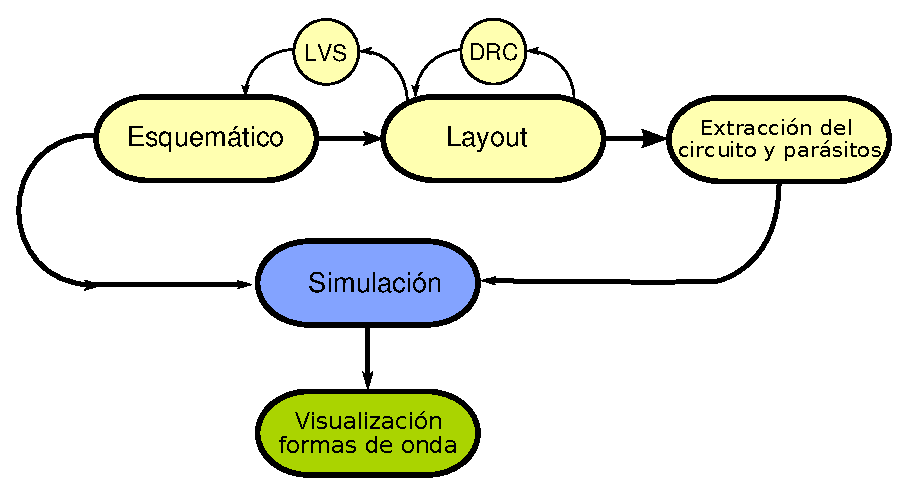
\includegraphics[scale=1.0]{figuras/analog-flow.eps}
  \caption{Flujo de diseño analógico.}
\label{fig:aflow}
%\vspace{-10pt}
\end{figure}
\section{Desafíos futuros}
Al realizar este proyecto integrador, hemos detectado la oportunidad de desarrollar líneas de trabajo en pos de profundizar algunos aspectos de la metodología o de la aplicación.  
\begin{itemize}
\item Crear un flujo que una los resultados esperados de \gls{pnr} con la selección de la arquitectura a implementar, de forma automática.
\item .
\item .
\end{itemize}




%El hecho de utilizar software libre genera una metodología de trabajo 


